\documentclass[11pt,a4paper]{article}

\usepackage[utf8]{inputenc}
\usepackage[T1]{fontenc}
\usepackage[english]{babel}
\usepackage{geometry}
\usepackage{microtype}
\usepackage{booktabs}
\usepackage{array}
\usepackage{longtable}
\usepackage{enumitem}
\usepackage{graphicx}
\usepackage{xcolor}
\usepackage{tikz}
\usepackage{pgfplots}
\usepackage{hyperref}
\usepackage[numbers,sort&compress]{natbib}
\usetikzlibrary{arrows.meta,positioning,fit,shapes.geometric,calc}
\pgfplotsset{compat=1.18}

\geometry{margin=2.6cm}
\setlist{noitemsep,topsep=4pt}

\newcommand{\llmind}{LLMind2}
\definecolor{llmblue}{HTML}{1F4E79}
\definecolor{llmcyan}{HTML}{D9EAF7}
\definecolor{llmgreen}{HTML}{DDEBDD}
\definecolor{llmorange}{HTML}{FCE4D6}
\definecolor{llmgray}{HTML}{F2F2F2}
\tikzset{
  box/.style={rounded corners, draw=llmblue, thick, fill=llmcyan, align=center, minimum height=0.9cm, text width=3.0cm, font=\small},
  data/.style={rounded corners, draw=black!55, thick, fill=llmgray, align=center, minimum height=0.9cm, text width=2.8cm, font=\small},
  agent/.style={rounded corners, draw=llmblue, thick, fill=llmgreen, align=center, minimum height=0.9cm, text width=2.8cm, font=\small},
  evalbox/.style={rounded corners, draw=black!60, thick, fill=llmorange, align=center, minimum height=0.9cm, text width=2.8cm, font=\small},
  arrow/.style={-{Latex[length=2.2mm]}, thick, draw=black!70}
}
\newcommand{\authoraction}[1]{%
  \vspace{0.6em}
  \noindent\framebox[\linewidth][l]{%
    \begin{minipage}{0.95\linewidth}
    \textbf{Author action required.} #1
    \end{minipage}}
  \vspace{0.6em}
}

\title{\textbf{\llmind: an ontology-grounded multi-agent framework for the scientific evaluation of diagnostic reasoning with Large Language Models in mental health}}

\author{
  Davide Ditolve\\
  \small Affiliation to be confirmed\\
  \small \texttt{email to be confirmed}
  \and
  Co-authors to be confirmed
}

\date{\today}

\begin{document}
\maketitle

\begin{abstract}
The use of Large Language Models (LLMs) in mental health requires evaluation methods that are substantially stricter than those commonly used for general-purpose conversational systems. The core risk is not only that a generated answer may be inaccurate, but that a system may produce untraceable nosological inferences, conflate non-equivalent diagnostic systems, or turn a research-support tool into an apparent clinical decision-maker. This paper presents \llmind, a research framework designed to study LLM-assisted diagnostic reasoning through three principles: explicit grounding in ICD-11 and the ICD-11 Clinical Descriptions and Diagnostic Requirements (CDDR), controlled benchmarking on DSM-5-TR clinical cases, and multi-agent decomposition aimed at separating intake, nosological coding, differential diagnosis, benchmark review, research methodology, and safety governance.

The proposal extends the previous LLMind Chat study, which demonstrated the feasibility of a Retrieval-Augmented Generation (RAG) approach over ICD-11 for supporting mental health professionals \citep{cremaschi2025decoding}. Version 2 shifts the emphasis from a single RAG assistant to a broader experimental environment, reproducible with local and open-source components, in which static sources are normalized into a queryable corpus, clinical cases are treated as versioned benchmark objects, conversational agents have explicit roles and guardrails, and evaluation combines automatic metrics, expert rubrics, and error analysis. The paper describes the scientific rationale, research questions, methodological design, conceptual architecture, planned evaluation protocol, and reproducibility strategy. Optional cloud integrations are treated only as deployment extensions, not as scientific prerequisites. \llmind\ is not presented as a diagnostic device, but as a reproducible environment for studying whether, how, and under which limitations LLMs can contribute to nosological reasoning in research and advanced clinical education.
\end{abstract}

\noindent\textbf{Keywords:} Large Language Models; Retrieval-Augmented Generation; ICD-11; DSM-5-TR; mental health; conversational agents; clinical benchmark; human-in-the-loop evaluation; clinical decision support.

\section{Introduction}
The classification of mental disorders requires the integration of heterogeneous information: reported symptoms, duration, functional impairment, course, differential diagnosis, medical or substance-related exclusions, cultural context, and risk level. Unlike other medical domains in which an instrumental signal may carry decisive diagnostic weight, psychology and psychiatry often rely on an interpretive process distributed across clinical interview, observation, history, diagnostic criteria, and professional judgement. Manuals such as DSM-5-TR and ICD-11 provide shared terminology and systematic criteria, yet their application remains a complex task \citep{apa2022dsm5tr,who2022icd11,who2024cddr}. The complexity increases when reasoning must cross non-identical classification systems, for example when DSM-5-TR cases are used to evaluate suggestions grounded in ICD-11.

This makes mental health a particularly relevant test case for evaluating LLMs. A model may generate a linguistically plausible answer even when it has not correctly identified the underlying clinical construct; it may omit essential exclusions, overinterpret insufficient information, or confuse semantic similarity with diagnostic equivalence. A scientific evaluation therefore cannot be limited to whether the name of a diagnosis appears in the output. It must evaluate the inferential path: which information was used, which information was ignored, which alternative hypotheses were considered, how uncertainty was stated, and which non-applicability conditions were recognized.

LLMs have shown remarkable capabilities in text generation, summarization, and medical question answering \citep{singhal2023medpalm,peng2023medical}. In mental health, however, the central issue is not merely the production of fluent responses. A scientifically useful system must make its anchors explicit, distinguish evidence from hypotheses, preserve source traceability, avoid definitive diagnoses on real cases, and support reproducible evaluation. The RAG literature suggests that access to non-parametric memory can improve factuality, updatability, and provenance \citep{lewis2020rag,li2022survey}. Yet retrieval alone does not solve the clinical reasoning problem: one must define what is retrieved, how it is structured, which agents use it, which outputs are allowed, and how the entire process is evaluated. In other words, the problem is not only architectural but epistemological: a reasoning-support system must make auditable the relationship between nosological source, clinical case, language model, and human judgement.

The previous LLMind Chat work proposed an ICD-11-based RAG system using Gemma 2 to support diagnostic reasoning in psychology and psychiatry, and evaluated it against DSM-5-TR clinical cases with expert validation \citep{cremaschi2025decoding}. That study showed that a general-purpose open model, when grounded in a specialized knowledge base, could provide more coherent suggestions than models not adapted to the task. Version 2 starts from a broader question: how can a RAG assistant be transformed into a scientific platform for experimenting with, comparing, and governing LLM-based diagnostic reasoning?

\llmind\ is designed as a research infrastructure. It does not aim to replace clinicians or provide operational diagnoses. Its purpose is to create a controlled environment in which to study the contribution of LLMs and conversational agents to ICD-11 coding, differential diagnosis, benchmark case review, methodological navigation, and safety control. In this perspective, the application interface is not the main contribution; it is a way to make reasoning processes observable, versionable, and evaluable rather than leaving them embedded in unstructured conversations. The scientific contribution is therefore twofold: a methodology for building a nosological corpus and controlled benchmark, and a protocol for evaluating not only the final answer but also the quality of the inferential process.

\section{From the original LLMind system to \llmind}
The original paper introduced LLMind Chat as a RAG application for ICD-11. The pipeline included extracting ICD-11 content through APIs, integrating ICD-11-CDDR, building textual prompts for each disorder, indexing them in a vector store, and querying a local LLM. Evaluation was conducted on DSM-5-TR clinical cases and compared the system against reference models \citep{cremaschi2025decoding}. Its main contribution was to show that an open model enriched with specialized retrieval could provide more relevant support in mental health reasoning.

\llmind\ preserves this intuition but changes the scientific question. Instead of asking only whether a single model answers a case correctly, the platform investigates which parts of the process contribute to reasoning quality. This distinction matters. An error may originate from an overly broad retrieval query, an unresolved DSM/ICD mapping, gold-standard leakage in the prompt, an overconfident generative answer, a weak evaluation rubric, or a failure to separate intake from differential reasoning. Version 2 therefore introduces functional decomposition.

The platform organizes the process into six agentic roles: clinical intake, ICD-11 coding, differential diagnosis supervision, benchmark case review, research protocol navigation, and safety governance. This organization does not imply that agents produce clinical truth. On the contrary, it is intended to make the interaction between sources, constraints, and outputs more verifiable. Each agent has a declared scope, expected inputs, allowed outputs, accessible sources, and handoff conditions.

\section{Research questions}
Version 2 is guided by four research questions.

\begin{enumerate}
  \item \textbf{RQ1 - Nosological grounding.} To what extent does explicit grounding in ICD-11/CDDR improve coherence, traceability, and appropriateness of suggestions compared with prompts without retrieval or with unstructured retrieval?
  \item \textbf{RQ2 - Multi-agent decomposition.} Does the separation between intake, coding, differential diagnosis, benchmark review, and safety reduce scope errors, leakage, and overclaiming compared with a single generalist assistant?
  \item \textbf{RQ3 - Cross-nosological evaluation.} What limitations emerge when DSM-5-TR cases are used to evaluate ICD-11-grounded outputs, and how can such limitations be modeled within the experimental protocol?
  \item \textbf{RQ4 - Reproducibility.} Can a static, normalized, and versioned corpus, queryable through local and open-source tools, support a reproducible agentic pipeline without sacrificing scientific auditability?
\end{enumerate}

\authoraction{Confirm whether these four research questions match the intended doctoral contribution. If the paper targets a specific journal or conference, length, framing, and priority of the RQs should be adapted to that venue.}

\section{Background}
\subsection{LLMs and mental health}
Research on LLMs in medicine has shown promising results in question answering, clinical summarization, and textual reasoning \citep{singhal2023medpalm,peng2023medical}. Mental health, however, has specific characteristics. Diagnoses are often syndromic, depend on temporal course, require medical and cultural exclusions, and are sensitive to the quality of information collection. Moreover, comorbidity and symptom overlap make a purely classificatory approach insufficient. A clinical vignette may contain signals compatible with multiple hypotheses; some information may be absent; other information may be ambiguous or depend on the way the case was narrated. In such contexts, a useful output is not necessarily one that immediately produces a diagnosis, but one that organizes the problem, identifies uncertainty, suggests plausible differentials, and clarifies which data would be required to proceed.

In this context, an LLM may be useful as a tool for structuring, exploration, and comparison, but risky if it produces assertive conclusions without making uncertainty, missing data, and exclusions explicit. The clinical LLM literature therefore emphasizes the need for human supervision, external evaluation, and a clear distinction between benchmark performance and real clinical validity \citep{singhal2023medpalm}. This is central to \llmind: the system is designed to measure and expose the conditions of reliability, not to hide uncertainty behind natural conversation.

\subsection{ICD-11, ICD-11-CDDR, and DSM-5-TR}
ICD-11 is the international classification of the World Health Organization, whereas DSM-5-TR is the manual of the American Psychiatric Association \citep{who2022icd11,apa2022dsm5tr}. Both are central to practice and research, but they are not interchangeable. ICD-11-CDDR provides clinical descriptions and diagnostic requirements for mental, behavioural, and neurodevelopmental disorders \citep{who2024cddr}. DSM-5-TR Clinical Cases provides structured vignettes useful for evaluating reasoning over clinical cases \citep{apa2023clinicalcases}.

Using DSM-5-TR cases to evaluate an ICD-11-grounded system creates a productive but delicate methodological tension. On the one hand, DSM cases provide benchmark material with gold standards. On the other hand, the gold standard does not necessarily correspond one-to-one to ICD-11 formulations. \llmind\ treats this tension as an explicit part of the experimental design rather than as a technical detail.

\subsection{Retrieval-Augmented Generation and external memory}
RAG combines a generative model with indexed external memory, allowing the system to retrieve relevant content before generation \citep{lewis2020rag}. In the clinical domain, this paradigm is especially useful because it separates model parameters from specialized knowledge and reduces reliance on the internal memory of the LLM. However, RAG does not guarantee correctness: irrelevant retrieval, suboptimal chunking, conflict between sources, and unfaithful generation remain open problems \citep{li2022survey}.

\subsection{Conversational agents and decomposition of reasoning}
Agentic orchestration is interpreted here in methodological terms: not as an arbitrary multiplication of chatbots, but as a controlled separation of epistemic responsibilities. An intake agent should not diagnose; an ICD-11 agent should not automatically translate DSM labels into ICD codes; a benchmark agent should not change a gold standard without human review; a guardrail should not continue clinical reasoning when acute risk or identifiable data are present. Decomposition enables the evaluation of specific failure modes and reduces confusion between tasks.

\section{Materials and sources}
\subsection{ICD-11 corpus}
The ICD-11 corpus is obtained through APIs and organized as a local taxonomy. For \llmind, the primary focus is Chapter 6, covering mental, behavioural, and neurodevelopmental disorders. Unlike legacy pipelines based on static intermediate files, version 2 assumes that primary extraction occurs through APIs and that the local base is then normalized into queryable tables. Each category should preserve, where available, code, title, description, hierarchical relations, inclusions, exclusions, index terms, and research-relevant metadata. This representation allows ICD-11 to be treated not as a simple text document, but as a navigable nosological structure.

The choice to extract ICD-11 through APIs has a scientific motivation: it reduces ambiguity introduced by manual conversions, makes extraction repeatable, preserves the link to original entity identifiers, and allows the study to distinguish taxonomic content from descriptive content. In benchmarking, this distinction matters because it helps determine whether the model is retrieving an appropriate category, using relevant diagnostic requirements, or merely generating a plausible paraphrase.

\subsection{ICD-11-CDDR}
ICD-11-CDDR is used as a textual source for clinical descriptions, diagnostic requirements, boundaries with normality, exclusions, and differentials. In the experimental design, CDDR is the main nosological reference for the ICD-11 and differential-diagnosis agents. Its role differs from the ICD-11 taxonomy: while the taxonomy provides identifiers, hierarchies, and categories, CDDR provides the clinical content that makes the category interpretable. For this reason, the corpus must preserve links between category, diagnostic description, and textual sections, avoiding retrieval of fragments detached from context.

\subsection{DSM-5-TR cases}
DSM-5-TR Clinical Cases are used as benchmark material and not as an ICD-11 truth source. Each case should be separated into distinct fields: presentation or introduction, discussion, diagnosis, and metadata. This separation is essential to avoid leakage: if the model receives the discussion or diagnosis during testing, the benchmark no longer measures diagnostic reasoning but contaminated information recovery.

The value of DSM-5-TR cases is twofold. On the one hand, they provide sufficiently structured clinical vignettes for comparable model testing. On the other hand, they introduce a methodological tension because the gold standard is formulated in a diagnostic system different from the primary grounding system. This tension should not be artificially removed; it should be measured. \llmind\ can therefore distinguish correctness with respect to the DSM gold standard, plausibility of mapping to ICD-11, and quality of differential reasoning.

\subsection{Static and reproducible corpus}
Version 2 introduces a static and versioned corpus, queryable through local and open-source tools. The motivation is not merely engineering-related. From a scientific perspective, a controlled tabular or document corpus makes it possible to:
\begin{itemize}
  \item freeze a specific version of the sources;
  \item reproduce the queries or searches performed by agents;
  \item measure which sections were retrieved;
  \item separate structured retrieval from generation;
  \item reduce uncontrolled variation across runs.
\end{itemize}

The unified agent chunk representation may include fields such as corpus, diagnostic family, section, code, text, source hash, and extraction version. This structure enables experiments in which an agent consults either the entire Chapter 6 or selected sections only, supporting a study of the trade-off between context breadth and retrieval precision. Cloud implementations, including possible export to BigQuery or managed conversational agents, may be useful for scaling the prototype or for application demonstrations, but they are not the scientific core of the paper because they are not necessarily reproducible for free or with open tools.

\begin{figure}[htbp]
\centering
\resizebox{\linewidth}{!}{%
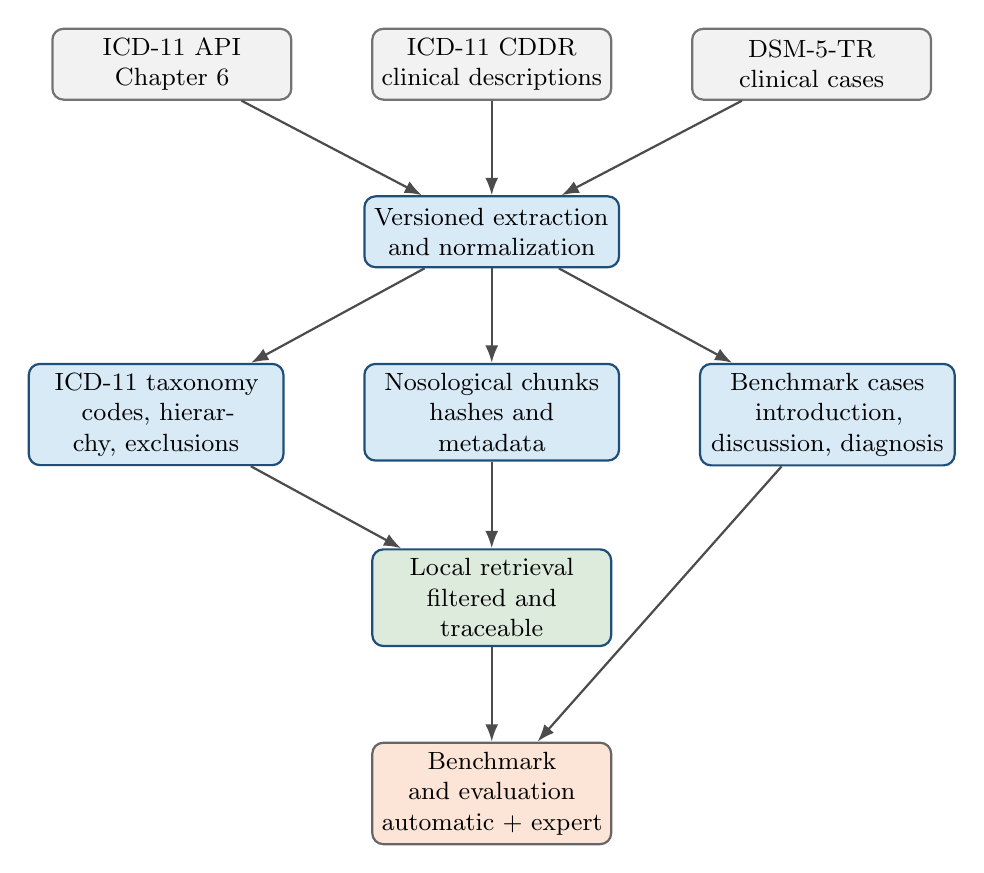
\begin{tikzpicture}[node distance=1.2cm and 1.0cm]
  \node[data] (icdapi) {ICD-11 API\\Chapter 6};
  \node[data, right=of icdapi] (cddr) {ICD-11 CDDR\\clinical descriptions};
  \node[data, right=of cddr] (dsm) {DSM-5-TR\\clinical cases};
  \node[box, below=of cddr] (extract) {Versioned extraction\\and normalization};
  \node[box, below left=of extract] (taxonomy) {ICD-11 taxonomy\\codes, hierarchy, exclusions};
  \node[box, below=of extract] (chunks) {Nosological chunks\\hashes and metadata};
  \node[box, below right=of extract] (cases) {Benchmark cases\\introduction, discussion, diagnosis};
  \node[agent, below=1.1cm of chunks] (retrieval) {Local retrieval\\filtered and traceable};
  \node[evalbox, below=of retrieval] (evaluation) {Benchmark and evaluation\\automatic + expert};

  \draw[arrow] (icdapi) -- (extract);
  \draw[arrow] (cddr) -- (extract);
  \draw[arrow] (dsm) -- (extract);
  \draw[arrow] (extract) -- (taxonomy);
  \draw[arrow] (extract) -- (chunks);
  \draw[arrow] (extract) -- (cases);
  \draw[arrow] (taxonomy) -- (retrieval);
  \draw[arrow] (chunks) -- (retrieval);
  \draw[arrow] (cases) -- (evaluation);
  \draw[arrow] (retrieval) -- (evaluation);
\end{tikzpicture}}
\caption{Reproducible corpus construction pipeline in \llmind. ICD-11, ICD-11-CDDR, and DSM-5-TR sources are transformed into versioned artifacts that can be queried locally while separating taxonomy, descriptive clinical content, and benchmark cases.}
\label{fig:data-pipeline-en}
\end{figure}

% BEGIN_DYNAMIC_ARTIFACT_SNAPSHOT_EN
\subsection{Numerical artifact snapshot}
To keep methodological contribution separate from experimental findings, this section reports a static snapshot of the artifacts available in the repository at the time of writing. These values are not clinical results. They are reproducibility counts: they describe the scale of the available corpus, benchmark cases, and agentic artifacts used by the protocol.

\begin{table}[htbp]
\centering
\begin{tabular}{lr}
\toprule
\textbf{Artifact} & \textbf{Count}\\
\midrule
Extracted ICD-11 categories & 720\\
Structured DSM-5-TR cases & 104\\
ICD-11 chunks for agent datastore & 523\\
DSM-5-TR chunks for agent datastore & 853\\
Total agent chunks & 1\,376\\
Conversational playbooks & 6\\
Defined subagents & 7\\
Source PDFs available for datastores & 3\\
\bottomrule
\end{tabular}
\caption{Quantitative snapshot of reproducible artifacts. Counts indicate the scale of the corpus and orchestration artifacts, not diagnostic performance.}
\label{tab:repo-snapshot-en}
\end{table}

\begin{figure}[htbp]
\centering
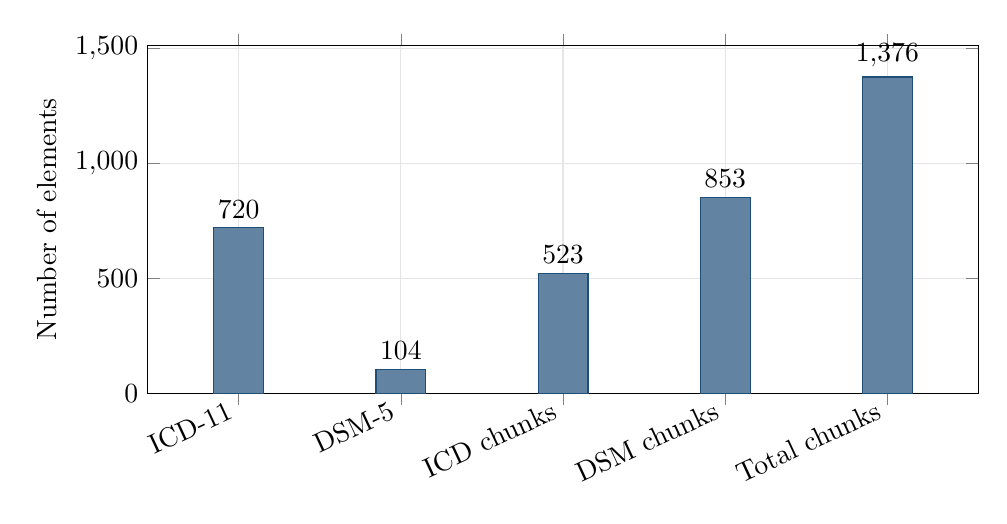
\begin{tikzpicture}
\begin{axis}[
  ybar,
  width=\linewidth,
  height=6cm,
  bar width=18pt,
  ymin=0,
  ylabel={Number of elements},
  symbolic x coords={ICD-11,DSM-5,ICD chunks,DSM chunks,Total chunks},
  xtick=data,
  x tick label style={rotate=25,anchor=east},
  nodes near coords,
  nodes near coords align={vertical},
  enlarge x limits=0.14,
  grid=major,
  major grid style={draw=black!10},
]
\addplot[fill=llmblue!70, draw=llmblue] coordinates {
  (ICD-11,720)
  (DSM-5,104)
  (ICD chunks,523)
  (DSM chunks,853)
  (Total chunks,1376)
};
\end{axis}
\end{tikzpicture}
\caption{Quantitative distribution of corpus artifacts. The chart highlights the separation between ICD-11 taxonomy, DSM-5-TR benchmark cases, and document chunks used by agents.}
\label{fig:repo-snapshot-chart-en}
\end{figure}
% END_DYNAMIC_ARTIFACT_SNAPSHOT_EN

\section{Research system design}
\subsection{Design principles}
\llmind\ follows five methodological principles:
\begin{enumerate}
  \item \textbf{Grounding before generation.} Every nosological output must be preceded by retrieval or consultation of structured sources.
  \item \textbf{Task separation.} Agents have limited and declared roles.
  \item \textbf{Experimental versioning.} Prompts, models, corpora, rubrics, and cases must be traceable.
  \item \textbf{Human-in-the-loop evaluation.} Expert validation is not optional when outputs concern clinical reasoning.
  \item \textbf{No clinical deployment claim.} The system is a research, education, and evaluation tool, not a medical device.
  \item \textbf{Local reproducibility.} Core components should be executable, inspectable, and replaceable in a controlled environment without dependence on proprietary services.
\end{enumerate}

\begin{figure}[htbp]
\centering
\resizebox{\linewidth}{!}{%
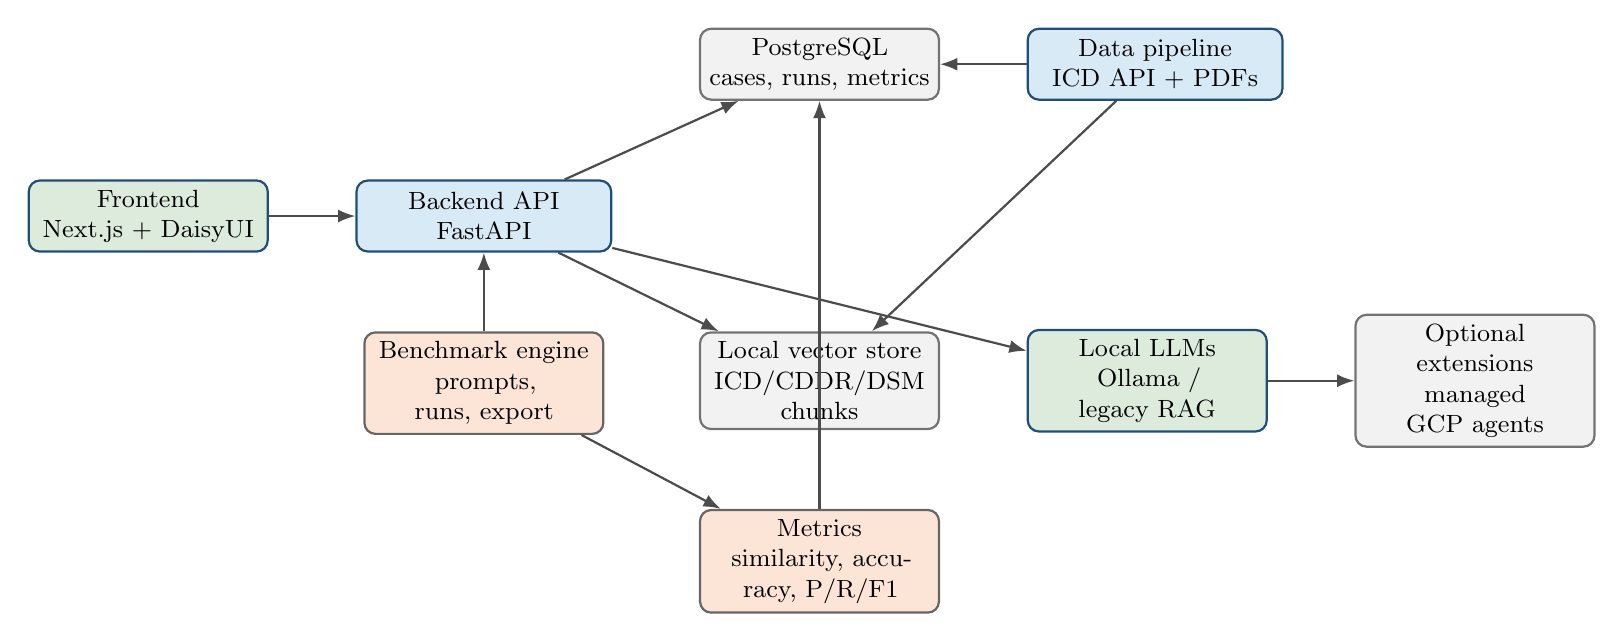
\begin{tikzpicture}[node distance=1.0cm and 1.1cm]
  \node[agent] (frontend) {Frontend\\Next.js + DaisyUI};
  \node[box, right=of frontend] (api) {Backend API\\FastAPI};
  \node[data, above right=of api] (postgres) {PostgreSQL\\cases, runs, metrics};
  \node[data, below right=of api] (vector) {Local vector store\\ICD/CDDR/DSM chunks};
  \node[box, right=of postgres] (etl) {Data pipeline\\ICD API + PDFs};
  \node[agent, right=of vector] (llm) {Local LLMs\\Ollama / legacy RAG};
  \node[evalbox, below=of api] (benchmark) {Benchmark engine\\prompts, runs, export};
  \node[evalbox, below=of vector] (metrics) {Metrics\\similarity, accuracy, P/R/F1};
  \node[data, right=of llm] (optional) {Optional extensions\\managed GCP agents};

  \draw[arrow] (frontend) -- (api);
  \draw[arrow] (api) -- (postgres);
  \draw[arrow] (api) -- (vector);
  \draw[arrow] (etl) -- (postgres);
  \draw[arrow] (etl) -- (vector);
  \draw[arrow] (api) -- (llm);
  \draw[arrow] (benchmark) -- (api);
  \draw[arrow] (benchmark) -- (metrics);
  \draw[arrow] (metrics) -- (postgres);
  \draw[arrow] (llm) -- (optional);
\end{tikzpicture}}
\caption{Implementation architecture of the local prototype. The reproducible core consists of the frontend, API, relational database, vector datastore, extraction pipeline, local LLMs, and benchmark engine. GCP integrations are optional deployment extensions rather than dependencies of the scientific protocol.}
\label{fig:system-architecture-en}
\end{figure}

\begin{figure}[htbp]
\centering
\resizebox{\linewidth}{!}{%
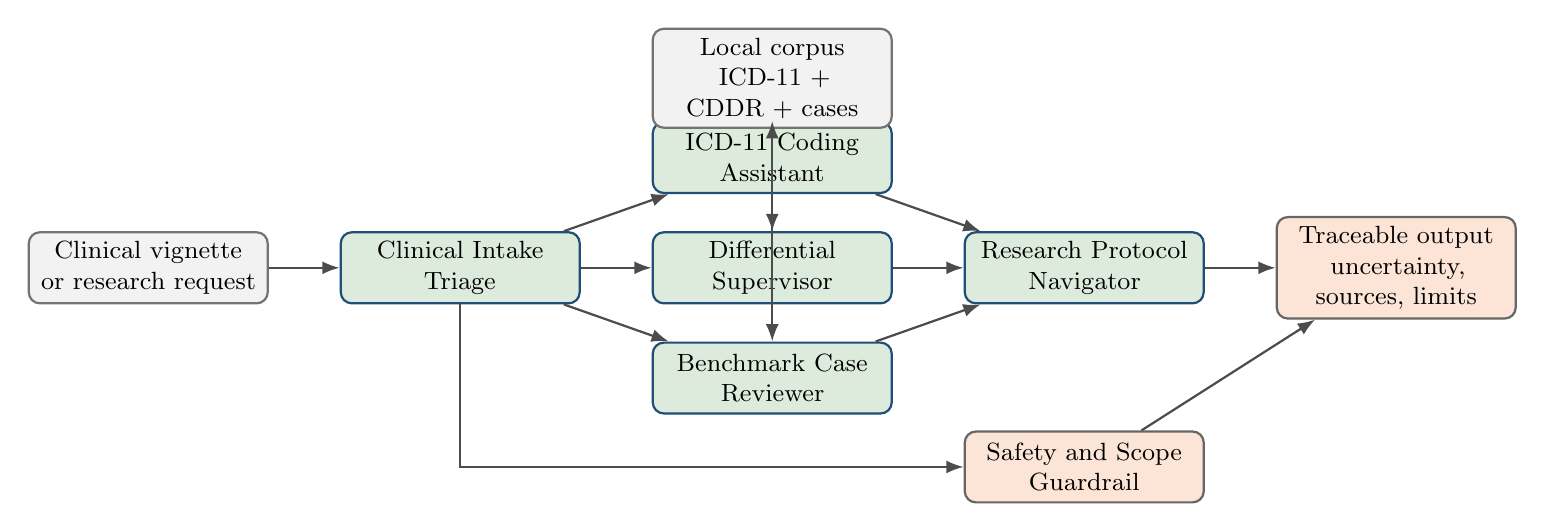
\begin{tikzpicture}[node distance=1.0cm and 0.9cm]
  \node[data] (case) {Clinical vignette\\or research request};
  \node[agent, right=of case] (intake) {Clinical Intake\\Triage};
  \node[agent, right=of intake, yshift=1.4cm] (coding) {ICD-11 Coding\\Assistant};
  \node[agent, right=of intake] (diff) {Differential\\Supervisor};
  \node[agent, right=of intake, yshift=-1.4cm] (bench) {Benchmark Case\\Reviewer};
  \node[agent, right=of diff] (protocol) {Research Protocol\\Navigator};
  \node[evalbox, below=1.6cm of protocol] (safety) {Safety and Scope\\Guardrail};
  \node[data, above=1.3cm of diff] (sources) {Local corpus\\ICD-11 + CDDR + cases};
  \node[evalbox, right=of protocol] (output) {Traceable output\\uncertainty, sources, limits};

  \draw[arrow] (case) -- (intake);
  \draw[arrow] (intake) -- (coding);
  \draw[arrow] (intake) -- (diff);
  \draw[arrow] (intake) -- (bench);
  \draw[arrow] (coding) -- (protocol);
  \draw[arrow] (diff) -- (protocol);
  \draw[arrow] (bench) -- (protocol);
  \draw[arrow] (protocol) -- (output);
  \draw[arrow] (safety) -- (output);
  \draw[arrow] (sources) -- (coding);
  \draw[arrow] (sources) -- (diff);
  \draw[arrow] (sources) -- (bench);
  \draw[arrow] (intake) |- (safety);
\end{tikzpicture}}
\caption{Conceptual multi-agent architecture. Decomposition is not a multiplication of chatbots, but the separation of epistemic responsibilities: case intake, nosological coding, differential diagnosis, benchmark review, protocol navigation, and safety.}
\label{fig:agent-architecture-en}
\end{figure}

\subsection{Planned agents}
\begin{longtable}{p{0.23\linewidth}p{0.31\linewidth}p{0.36\linewidth}}
\toprule
\textbf{Agent} & \textbf{Scientific function} & \textbf{Allowed output}\\
\midrule
Clinical Intake Triage & Structures the vignette, identifies missing data, and selects the next path. & Neutral summary, missing data, risk flags, handoff.\\
ICD-11 Coding Assistant & Retrieves candidate ICD-11 categories and diagnostic requirements. & ICD-11 candidates, evidence for/against, exclusions, uncertainty.\\
Differential Diagnosis Supervisor & Compares diagnostic hypotheses while keeping evidence and inference separate. & Differential table, must-not-miss conditions, next questions.\\
Benchmark Case Reviewer & Checks DSM case quality and leakage risk. & Case readiness, artifacts, contamination flags, human-review requests.\\
Research Protocol Navigator & Maintains methodological coherence across experiments. & Protocol, metrics, validity risks, next actions.\\
Safety and Scope Guardrail & Blocks direct clinical use, identifiable data, or acute-risk handling. & Safe response, human escalation, scope delimitation.\\
\bottomrule
\end{longtable}

\subsection{Experimental conditions}
The paper proposes comparing at least five conditions:
\begin{enumerate}
  \item base model without retrieval;
  \item model with unstructured RAG over ICD-11/CDDR;
  \item model with local static corpus and filtered retrieval;
  \item single generalist agent with access to the same sources;
  \item multi-agent orchestration with separated roles.
\end{enumerate}

These conditions make it possible to isolate the effect of grounding, corpus structuring, and agentic decomposition. The comparison should not be reduced to diagnostic accuracy alone, because a more cautious but less assertive system may be scientifically preferable to a system that guesses more often while producing fragile justifications. Any deployment on cloud platforms or managed conversational systems may be reported in an appendix or as a note on technological transferability, but it should not enter the main experimental conditions.

\section{Reproducibility}
Reproducibility is a central requirement of \llmind, not a secondary property of the software. The first LLMind study already emphasized the description of the dataset construction pipeline, model choice, RAG configuration, and evaluation over DSM-5-TR cases. Version 2 extends this approach by making explicit all elements that must be fixed before the experiment and preserved after execution. The goal is to allow an independent group to reconstruct not only the application, but the experimental design: which sources were used, how they were transformed, which prompts were submitted, which models responded, and how responses were evaluated.

\begin{figure}[htbp]
\centering
\resizebox{0.95\linewidth}{!}{%
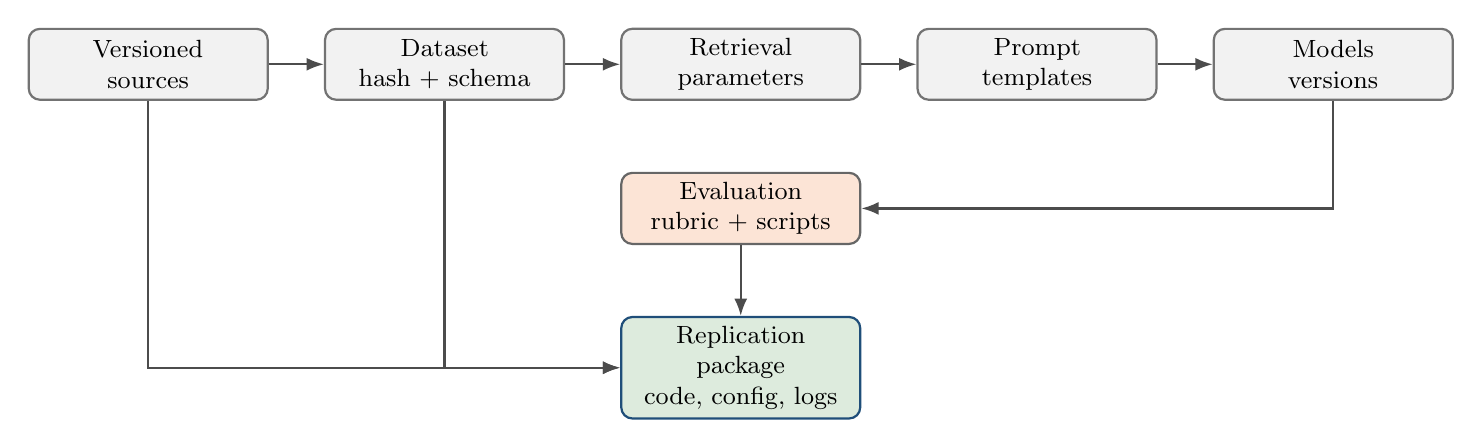
\begin{tikzpicture}[node distance=0.9cm and 0.7cm]
  \node[data] (sources) {Versioned\\sources};
  \node[data, right=of sources] (data) {Dataset\\hash + schema};
  \node[data, right=of data] (retrieval) {Retrieval\\parameters};
  \node[data, right=of retrieval] (prompts) {Prompt\\templates};
  \node[data, right=of prompts] (models) {Models\\versions};
  \node[evalbox, below=of retrieval] (eval) {Evaluation\\rubric + scripts};
  \node[agent, below=of eval] (package) {Replication package\\code, config, logs};

  \draw[arrow] (sources) -- (data);
  \draw[arrow] (data) -- (retrieval);
  \draw[arrow] (retrieval) -- (prompts);
  \draw[arrow] (prompts) -- (models);
  \draw[arrow] (models) |- (eval);
  \draw[arrow] (eval) -- (package);
  \draw[arrow] (sources) |- (package);
  \draw[arrow] (data) |- (package);
\end{tikzpicture}}
\caption{Reproducibility artifact chain. Every experimental result should be traceable to sources, datasets, retrieval settings, prompts, models, parameters, and evaluation procedures.}
\label{fig:reproducibility-en}
\end{figure}

\subsection{Data reproducibility}
Sources must be described with version, origin, and extraction procedure. For ICD-11, this means reporting API endpoint or container, extraction date, language, Chapter 6 filter, and schema of the resulting table. For ICD-11-CDDR, the study should report edition, source format, segmentation procedure, and criterion for linking descriptive text to diagnostic categories. For DSM-5-TR Clinical Cases, the procedure separating introduction, discussion, and diagnosis must be documented, because this step determines leakage risk and therefore benchmark validity.

Every transformed record should include a stable identifier, a hash of the source content or generated chunk, the name of the extraction pipeline, and the code version used. In this way, if a model answer is challenged, it becomes possible to trace the retrieved fragment and determine whether the error comes from the model, retrieval, data preparation, or gold standard.

\subsection{Retrieval and prompt reproducibility}
For each experimental condition, the study must preserve system prompts, user prompts, retrieval templates, number of retrieved documents, similarity thresholds, chunking strategy, embedding model, and generation parameters. In the multi-agent setting, it should also record which agent received the case, which handoff was activated, and which context was passed to the next agent. Without this traceability, two apparently identical runs may differ substantially.

Reproducibility does not necessarily require perfect determinism, which is often impossible with generative models. It does require that sources of variability are known and measured. For this reason, the protocol should fix temperature, top-p, seed when available, model version, and runtime version. When a model does not allow full seed control, the paper should state this and include repeated runs or stability analysis.

\subsection{Environment reproducibility}
The minimum reproducible environment should be local and based on inspectable tools: relational database for ICD-11 and cases, local vector index, versioned extraction scripts, local LLM runtime or open-weight model executable by third parties, and declarative configuration files. Docker or equivalent environments can fix dependencies, versions, and required services. Cloud deployment may be useful for scaling or demonstration, but it should not be required to reproduce the paper results.

\subsection{Evaluation reproducibility}
Evaluation must be as reproducible as the technical pipeline. The study should archive the list of included cases, exclusion criteria, experimental conditions, expert rubric, instructions to raters, response format shown to raters, and any randomization. Automatic metrics must be computed from versioned scripts, while manual evaluations should preserve score, rater, timestamp, and qualitative notes. When source material cannot be redistributed because of copyright, the paper should still describe procedures and schemas sufficiently for replication by researchers with legitimate access to the same sources.

\authoraction{Prepare a final ``Reproducibility artifacts'' table including: ICD-11 version, CDDR version, number of DSM cases, models, embeddings, generation parameters, data schema, prompt templates, rubric, number of raters, and code commit/tag.}

\section{Evaluation protocol}
\subsection{Experimental tasks}
Evaluation should include distinct tasks:
\begin{itemize}
  \item identification of candidate diagnoses from DSM-5-TR vignettes;
  \item mapping between DSM diagnoses and candidate ICD-11 categories;
  \item generation of differential diagnoses;
  \item detection of missing information;
  \item detection of case leakage;
  \item classification of out-of-scope or safety-sensitive requests.
\end{itemize}

\begin{figure}[htbp]
\centering
\resizebox{\linewidth}{!}{%
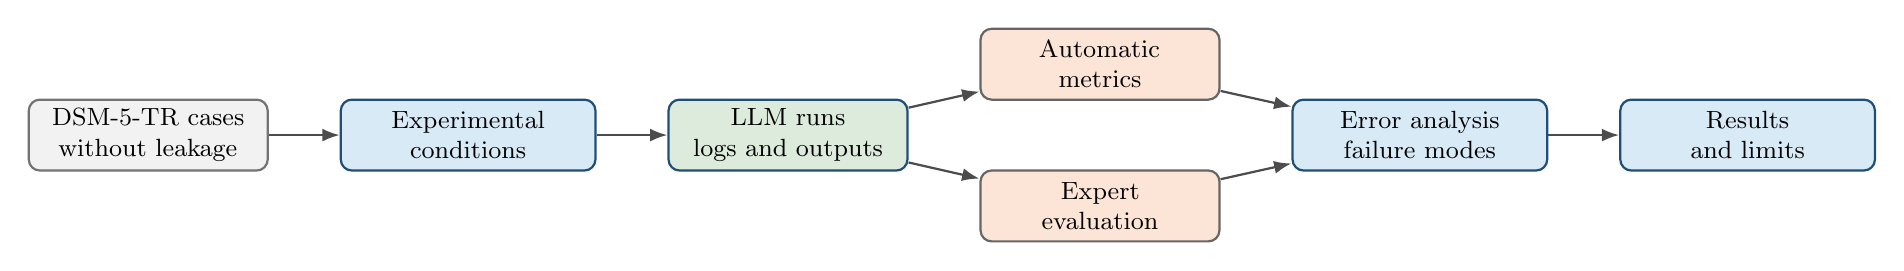
\begin{tikzpicture}[node distance=1.0cm and 0.9cm]
  \node[data] (cases) {DSM-5-TR cases\\without leakage};
  \node[box, right=of cases] (conditions) {Experimental\\conditions};
  \node[agent, right=of conditions] (runs) {LLM runs\\logs and outputs};
  \node[evalbox, right=of runs, yshift=0.9cm] (metrics) {Automatic\\metrics};
  \node[evalbox, right=of runs, yshift=-0.9cm] (raters) {Expert\\evaluation};
  \node[box, right=of metrics, yshift=-0.9cm] (errors) {Error analysis\\failure modes};
  \node[box, right=of errors] (report) {Results\\and limits};

  \draw[arrow] (cases) -- (conditions);
  \draw[arrow] (conditions) -- (runs);
  \draw[arrow] (runs) -- (metrics);
  \draw[arrow] (runs) -- (raters);
  \draw[arrow] (metrics) -- (errors);
  \draw[arrow] (raters) -- (errors);
  \draw[arrow] (errors) -- (report);
\end{tikzpicture}}
\caption{Evaluation workflow. Automatic metrics and expert evaluation are kept separate and then integrated in error analysis, avoiding reduction of diagnostic reasoning to accuracy alone.}
\label{fig:evaluation-workflow-en}
\end{figure}

\subsection{Automatic metrics}
In the prototype, automatic metrics are computed at the end of each benchmark run and stored together with the model response. Semantic similarity compares embeddings of the response and the gold-standard diagnosis. Label accuracy is a binary indicator based on exact textual containment or sufficient lexical overlap with the expected diagnosis. Precision, recall, and F1 are computed on normalized tokens from the response and the gold standard. The ``no diagnosis'' flag identifies empty or abstentive answers, distinguishing assertive error from failure to formulate a diagnosis. Latency and human evaluation are stored as complementary dimensions.

\begin{table}[htbp]
\centering
\begin{tabular}{p{0.22\linewidth}p{0.52\linewidth}p{0.18\linewidth}}
\toprule
\textbf{Metric} & \textbf{Operational definition} & \textbf{Implemented}\\
\midrule
Semantic similarity & Cosine similarity between response embedding and gold-standard embedding. & Yes\\
Label accuracy & 1 if the expected diagnosis appears in the response or lexical recall exceeds the threshold; 0 otherwise. & Yes\\
Precision & Share of diagnostic response tokens present in the gold standard. & Yes\\
Recall & Share of gold-standard diagnostic tokens recovered in the response. & Yes\\
F1 & Harmonic mean of precision and recall. & Yes\\
No diagnosis & Flag for empty, abstentive, or insufficient answers. & Yes\\
Top-k accuracy & Accuracy over a ranked list of diagnostic candidates. Requires structured candidate storage. & Planned\\
\bottomrule
\end{tabular}
\caption{Automatic benchmark metrics. Lexical measures are reproducible heuristics and must be interpreted together with expert evaluation rather than as evidence of clinical validity.}
\label{tab:automatic-metrics-en}
\end{table}

\subsection{Expert evaluation}
Expert evaluation should use a multidimensional rubric:
\begin{itemize}
  \item coherence with the case;
  \item nosological appropriateness;
  \item quality of differential diagnosis;
  \item explicitness of exclusions and missing data;
  \item calibration of uncertainty;
  \item absence of clinical overclaiming;
  \item usefulness for research or education.
\end{itemize}

Inter-rater agreement can be estimated using concordance indices, for example the concordance correlation coefficient where appropriate \citep{barnhart2002ccc}. The rubric must be defined before the experiment rather than adapted after observing results.

\authoraction{At least two expert raters are needed, or alternatively a strong methodological justification for single-rater evaluation. The rubric scale must be decided: binary, Likert 1--5, or continuous 0--1 as in the previous work.}

\subsection{Error analysis}
Error analysis should distinguish clinically and methodologically meaningful categories:
\begin{itemize}
  \item missing candidate diagnosis;
  \item correct diagnosis with incorrect justification;
  \item DSM/ICD confusion;
  \item missing exclusion;
  \item undetected missing information;
  \item prompt leakage;
  \item hallucinated code or criterion;
  \item overassertive response;
  \item safe but unhelpful response.
\end{itemize}

This taxonomy allows the study to assess whether multi-agent orchestration reduces specific errors even when it does not immediately improve aggregate accuracy.

\section{Hypotheses}
The main hypotheses are:
\begin{enumerate}
  \item ICD-11/CDDR grounding improves nosological quality compared with ungrounded prompts.
  \item Filtered retrieval over a static corpus reduces noise and cost compared with unstructured document retrieval.
  \item Multi-agent decomposition reduces overclaiming and leakage compared with a generalist agent.
  \item Expert evaluation will reveal divergences between label correctness and reasoning quality, making accuracy alone insufficient.
\end{enumerate}

\section{Ethics and governance}
\llmind\ must be interpreted as a research platform. Use with real patients, identifiable data, or risk situations requires external procedures, ethical approvals, and qualified supervision. The boundary must be explicit in the paper: the system supports study, benchmarking, and methodological analysis; it does not produce clinical diagnoses and does not replace professional evaluation.

Data governance is central. DSM-5-TR cases are copyrighted material and must be handled according to license and permitted purpose. ICD-11 and CDDR sources must be cited properly. The recommended experimental configuration is local or otherwise controlled, in order to minimize data transfers to third-party services. Any interaction with cloud agents should be considered extra-protocol, avoid personal data, and include logging, minimization, and access control. If real clinical data are used in the future, a dedicated ethical protocol will be required, including de-identification, legal basis, data protection impact assessment, and institutional review.

\authoraction{State explicitly whether version 2 uses only published/synthetic cases or also real clinical data. If real data are planned, ethical approval is required before any experiment.}

\section{Expected results and analysis plan}
This draft does not report new empirical results because the experimental phase of version 2 still has to be completed. The paper is therefore structured as the basis for an empirical study: the results sections should be populated after benchmark execution.

Results should be organized into four blocks:
\begin{enumerate}
  \item diagnostic and nosological performance by experimental condition;
  \item expert evaluation of reasoning quality;
  \item error analysis and failure modes;
  \item latency, local computational cost, and reproducibility of agentic queries.
\end{enumerate}

\authoraction{After the first experimental run, insert: number of cases, tested models, retrieval configuration, corpus version, number of raters, aggregate metrics, confidence intervals if available, and at least three qualitative examples of success/failure.}

\section{Threats to validity}
\subsection{Internal validity}
The main internal threat is leakage. If elements of the diagnosis or discussion enter the prompt, evaluation overestimates model ability. A second threat concerns retrieval variability: different corpus versions or chunking parameters may change outputs. A third threat is the non-determinism of generative models.

\subsection{External validity}
DSM-5-TR cases are published educational cases. They do not necessarily represent the distribution of complexity, incompleteness, and ambiguity found in real cases. Moreover, results on vignettes do not imply clinical performance in operational settings.

\subsection{Construct validity}
Diagnostic accuracy does not fully measure reasoning quality. An output may contain the correct label but a flawed rationale; conversely, it may be clinically cautious while not producing a specific label. For this reason, evaluation must include qualitative and safety-oriented dimensions.

\subsection{Conclusion validity}
Small samples, a limited number of raters, and DSM/ICD differences may limit generalizability. Conclusions should therefore be framed in terms of experimental support rather than clinical efficacy.

\section{Expected contributions}
The scientific contribution of version 2 can be summarized in four points:
\begin{enumerate}
  \item a framework for studying ontology-grounded LLMs in mental health;
  \item a benchmark protocol distinguishing label accuracy, reasoning quality, and safety;
  \item a multi-agent orchestration proposal with separated epistemic roles;
  \item a locally reproducible static and versioned corpus strategy for making retrieval and evaluation more controllable.
\end{enumerate}

\section{Conclusion}
\llmind\ extends LLMind Chat by transforming a RAG assistant into a research platform for LLM-assisted diagnostic reasoning. The central point is not to show that a model can replace a professional, but to study under which conditions nosological grounding, corpus structuring, agentic orchestration, and human-in-the-loop evaluation can make the use of LLMs more transparent, controllable, and scientifically evaluable.

Version 2 proposes a relevant conceptual shift: from chatbot as interface to system as laboratory. In a high-epistemic-risk domain such as mental health, this shift is essential. Only by separating sources, tasks, constraints, and metrics is it possible to understand whether LLMs truly contribute to reasoning quality or merely produce linguistically plausible explanations. Future work will execute the protocol, complete expert validation, publish reproducible results, and evaluate the impact of multi-agent decomposition on the most critical failure modes.

\section*{Quick checklist to complete the paper}
\begin{enumerate}
  \item Confirm title, authors, affiliations, and target venue.
  \item Decide which models will be compared in version 2.
  \item Run benchmarks on DSM-5-TR cases under the defined experimental conditions.
  \item Involve expert raters and freeze the rubric before evaluation.
  \item Add quantitative results, qualitative examples, and error analysis.
  \item Verify licenses and permissions for citing or describing DSM-5-TR cases.
  \item Decide whether to include figures: conceptual architecture, agent flow, evaluation protocol.
\end{enumerate}

\bibliographystyle{plainnat}
\bibliography{references}

\end{document}
